\enteteExam{NFP 107 -- Systèmes de gestion de bases de données - Durée 2h30}%
{Examen FOAD session 1}%
{Les documents ne sont pas autorisés}%

On s'intéresse au système d'information d'une station de ski. Elle propose
des remontées mécaniques pour accéder à des pistes. Une piste
peut être desservie par plusieurs remontées, et une remontée peut desservir 
plusieurs pistes.
La station propose
aux skieurs d'accéder à chaque remontée mécanique moyennant un tarif 
appliqué à chaque passage. 
Un cumul des passages par skieur est effectué
                 en fin de journée, et le montant obtenu
                est prélevé sur le compte du skieur.

Un concepteur propose le schéma suivant; les clés primaires sont en gras.

\begin{itemize}
\item Skieur(\textbf{id}, nom, prénom, noMobile)
\item Remontée (\textbf{id}, intitulé, tarif)
\item Passage(\textbf{id}, jour, heure, idSkieur, idRemontée)
\item Piste(\textbf{id}, nom, couleur, longueur)
\item AccèsPiste(\textbf{idRemontée, idPiste})

\end{itemize}

\subsection*{Conception du schéma (6 pts)}

\begin{enumerate}
   \item Donnez la liste des clés étrangères.

 \item Aurait-on pu choisir comme clé de la table \texttt{Passage}
      la paire d'attributs (idSkieur, idRemontée)\,? Donnez vos arguments pour ou contre
      un tel changement.
       
  \item Le schéma permet-il de savoir sur quelles pistes est passé un skieur?
  
 \item Donnez les commandes SQL de création des tables \texttt{Remontée}, \texttt{Piste}
 et \texttt{AccèsPiste}.

  \item Indiquez comment exprimer la contrainte suivante\,:
         deux skieurs différents ne peuvent pas avoir le même
             numéro de mobile.

  \item Quel est d'après vous le schéma entité-association 
        correspondant à ce schéma relationnel\,?
        
%   \item Chaque remontée mécanique est attribuée à un employé de la station
%    qui se charge de l'entretien, du contrôle des skieurs,
%     et de l'assistance éventuelle. Plusieurs
%     employés peuvent être affectés aux remontées à fort débit, 
%     
%     Proposez une extension du schéma relationnel et du schéma E/A pour
%     ajouter les employés et leur affectation.

\end{enumerate}

   
\begin{solution}
La figure~\ref{station} montre le schéma E/A, avec les employés. NB\,:
on peut envisager de créer une seule entité regroupant les skieurs
et les employés (qui ont le droit sans doute de skier
pendant leur période de congé). 

  \begin{figure}[htb]  
   \centerline{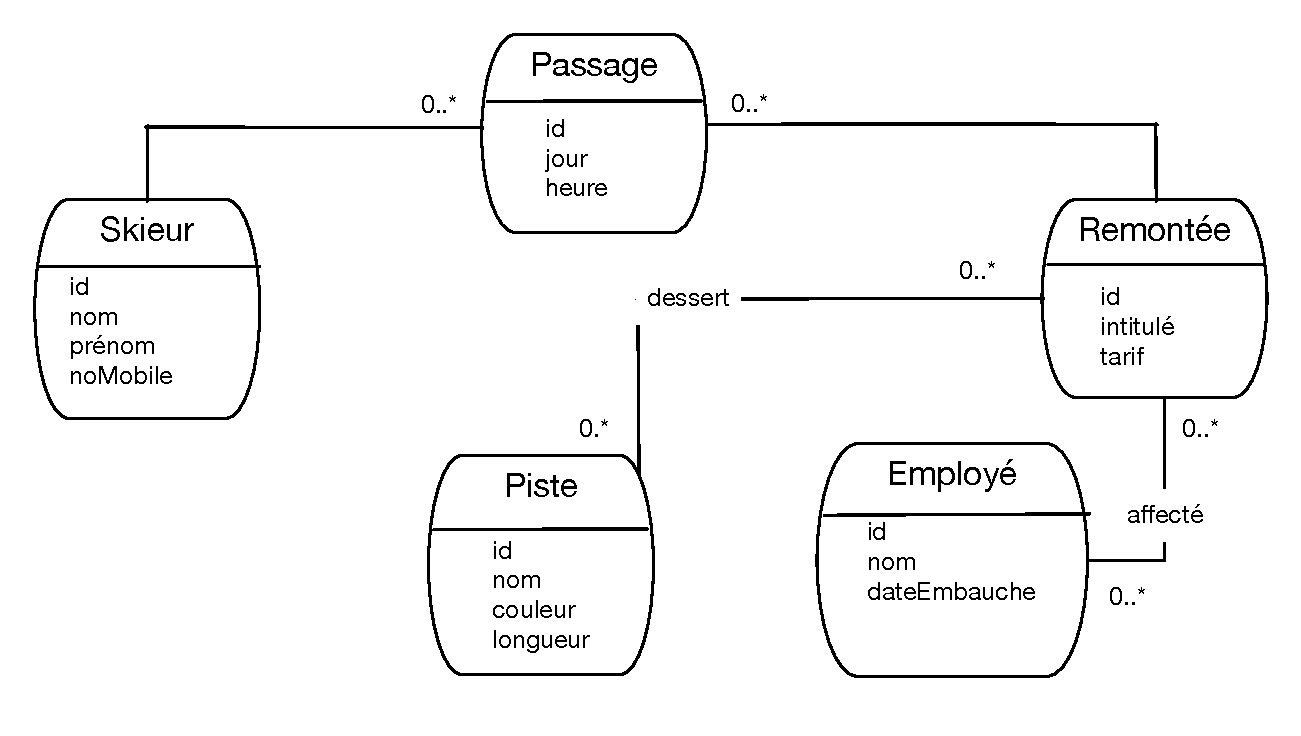
\includegraphics[scale=0.5]{../supports/figures/exam-20-stationski}}
    \caption{Modèle de la station de ski}  
    \label{station}  
  \end{figure}  
\end{solution}


\subsection*{SQL (7 pts)}

Sur le schéma obtenu précédemment, exprimez en SQL les requêtes suivantes\,:

\begin{enumerate}
  \item Id des remontées empruntées par le skieur Gilles Carpet.
  
   \item Intitulé des remontées donnant accès aux pistes dont la longueur est 
         supérieure à 1\,500 m. 

   \item Quels skieurs (prénom, nom) n'ont jamais pris la remontée intitulée "Marmottes"\,?

%   \item Donner la longueur totale et la longueur moyenne des pistes noires.

   \item Quelles sont les remontées  (intitulé, tarif)
    donnant accès à la piste \guill{Pylones}\,?
   
%   \item Combien de skieurs s'appellent \guill{Jean Renard}
%           parmi ceux qui ont  pris la remontée  \guill{Génépi}\,?

   \item Quelle est la requête donnant, pour chaque skieur
        et chaque jour de son séjour, son nom, 
       le nombre de remontées empruntées et le cumul des tarifs.
\end{enumerate}


\begin{solution}
\begin{minted}{sql}
select idRemontée 
from  Passage as p, Skieur as s
where s.prénom='Gilles' and s.nom='Carpet'
and p.idSkieur = s.id
\end{minted}

\begin{minted}{sql}
select intitulé 
from  Remontée as r, Piste as p, AccèsPiste as a 
where r.id = a.idRemontée 
and p.longueur > 1500
\end{minted}

\begin{minted}{sql}
select prénom, nom
from  Skieur 
where id not in (select idSkieur
              from Remontée as r, Passage as p
                p.idRemontée = r.id
                and r.intitulé = 'Marmottes' )
\end{minted}

\begin{minted}{sql}
select count(*)
from  Skieur as s, Remontée as r, Passage as p
where  p.idRemontée = r.id
and s.id = p.idSkieur
and r.intitulé = 'Génépi' 
and s.nom='Renard' and s.préniomp='Jean'
\end{minted}


\begin{minted}{sql}
select  s.nom, p.jour, count(*)
from  Skieur as s, Remontée as r, Passage as p
where  p.idRemontée = r.id
and s.id = p.idSkieur
group by s.id, p.jour
\end{minted}



\end{solution}



\subsection*{Algèbre (2 pts)}

Donnez les expressions algébriques correspondant aux deux premières requêtes SQL ci-dessus.


\subsection*{Vues (3 pts)}

\begin{enumerate}
   \item Créez une vue \texttt{Fréquentation} donnant, pour chaque
         remontée et chaque jour, le nombre de fois où la remontée 
             a été empruntée.
     \item A-t-on le droit d'insérer dans cette vue\,? Expliquez.
     
      \item En utilisant cette vue, quelle requête donne les remontées
         qui ont été empruntées plus de 5\,00 fois en une seule journée.
\end{enumerate}


\subsection*{Procédures (2 pts)}

\begin{enumerate}

  \item Rappeler quelles sont les trois phases d'utilisation d'un curseur.
  \item Expliquer ce que signifie l'immuabilité d'un curseur.
 
\end{enumerate}

\end{document}


\subsection*{Indexation (3 pts)}

\`A la fin de la saison, 250\,000 skieurs
ont fréquenté la station. On stocke
les données dans une base ORACLE avec des blocs
de 4\,000 octets, et on 
suppose que chaque ligne de la table \texttt{Skieur} occupe
200 octets sur le disque. 
 Répondez aux questions suivantes en justifiant
    vos réponses (on suppose que les pages sont pleines
   et on ne tient pas compte de la mémoire cache).
  \begin{enumerate}
   \item Quelle est la taille du segment de données pour 
           la table \texttt{Skieur} (en blocs, et en octets)\,? 


  \item L'identifiant du skieur est un entier sur 4 octets,
         et l'adresse d'un bloc occupe 16 octets. Décrivez
          la structure de l'arbre B+ sur l'id, et donnez son nombre de niveaux
         en fonction des chiffres précédents. 

  \item En supposant qu'il faut 10ms pour lire un bloc, 
         quel est le temps {\em moyen} de recherche d'un skieur
         par son identifiant GPS en supposant qu'il n'y a pas d'index\,?
       Quel est le temps d'accès à un skieur en fonction de son id\,?

\begin{solution}
\begin{enumerate}
  \item 50 Mo!
  \item $\frac{50000000}{4000}=12500$
\end{enumerate}
\end{solution}
\begin{solution}
   \item Quelle est la taille d'un index de type arbre-B
        si la clé fait 32 octets
           et un pointeur 8 octets\,?

Une entrée d'index fait 40 octets. Donc on en met
$\frac{4000}{40}=100$ par page. Il faut indexer 1\,000\,000
enregistrements pour le dernier niveau de l'index, soit
$\frac{1000000}{100}=10000$ pages. Ensuite il
faut indexer chacune des 1000 pages, soit $\frac{1000}{100}=10$
pages supplémentaires, que pour finir on indexe avec la racine.

Donc il faut 10000 + 10 + 1 pages dans l'index.
\end{solution}
 \begin{solution}
 
   \item  Si on suppose qu'un E/S coûte 10 ms, quel est le coût moyen
    d'une recherche
     d'un enregistrement par clé unique,
   avec index et sans index\,?


Recherche avec index\,: trois lectures dans l'index, 
puis une lecture dans le fichier. Soit 40 ms.

Sans index, en moyenne il faut lire la moitié du fichier,
soit 5625 pages, soit plus de 50 secondes.
\end{solution}
\end{enumerate}


\subsection*{\'Evaluation de requêtes (3 pts)}

On veut donner le nom de toutes les remontées
mécaniques qui sont de type \guill{Téléski}. Bien entendu, on suppose
que la table stockant les types est considérablement plus petite
que la table stockant les remontées.

\begin{enumerate}
   \item Donner la requête SQL.
   \item Donner l'expression algébrique correspondante.
    \item Donner au moins deux plans d'exécution possibles, sous la 
             forme qui vous convient.
          Quel est le meilleur d'après vous\,? Quels
     index peut-on créer pour améliorer les performances de cette requête\,?

\end{enumerate}
